


\section{Question 1}
\label{part1}

Choose 100 URIs from Assignment1 and generate WARC files of those URIs using:
	
\begin{itemize}
\item wget
	  ,WARCreate
	  ,Heritrix (stand-alone or via WAIL)
	  and webrecorder.io
\item Describe the resulting WARC files: quantitavely compare and contrast the results of the 
	  WARC files of the same URI as generated by different tools
	  	- choose interesting examples
\item Demonstrate playback of 2-3 WARCs in the (Wayback Machine (via WAIL or stand-alone) or pywb) 
	 and (webrecorder.io)
	  -``\url{https://github.com/iipc/openwayback}''
	  -``\url{https://github.com/ikreymer/pywb}''
\end{itemize}
\subsection{Solution}

The following steps were taken to setup tools and generate WARC files:
\begin{itemize}
	\item Installed wget using 'brew install wget'.
	\item WARC file for each URI is generated using the command 'wget --warc-file=outputfilename link'.
	\item Downloaded WARCreate chrome extension from chrome web store and added it to the chrome browser. Generated WARC for each 
		  URI manually by providing input to WARCreate.
		
	\item Installed WAIL.
	\item The figure below shows how to generate warc files for multiple URIs using single heritrix instance.
	\item When a URI had parameters then WAIL wasn't able to generate warc file.
		  \begin{figure}
		  	 \begin{center}
		  	 		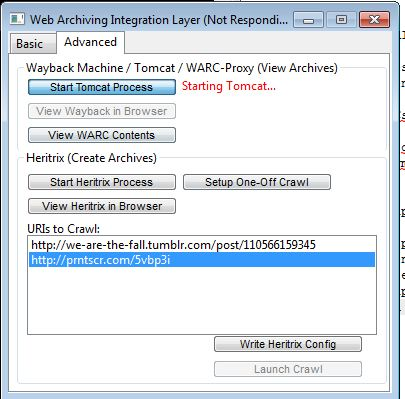
\includegraphics[scale=0.60]{WarcUsingWAIL.jpg}
		  	 		\caption{Generating warc files for multiple URIs using WAIL}
			  \end{center}
		  \end{figure}
	\newpage
	
	\item Used ``\url{https://webrecorder.io/}'' . Generating warc files for multiple URIs is done as shown in the figure below.
		\begin{figure}
		  	 \begin{center}
		  	 		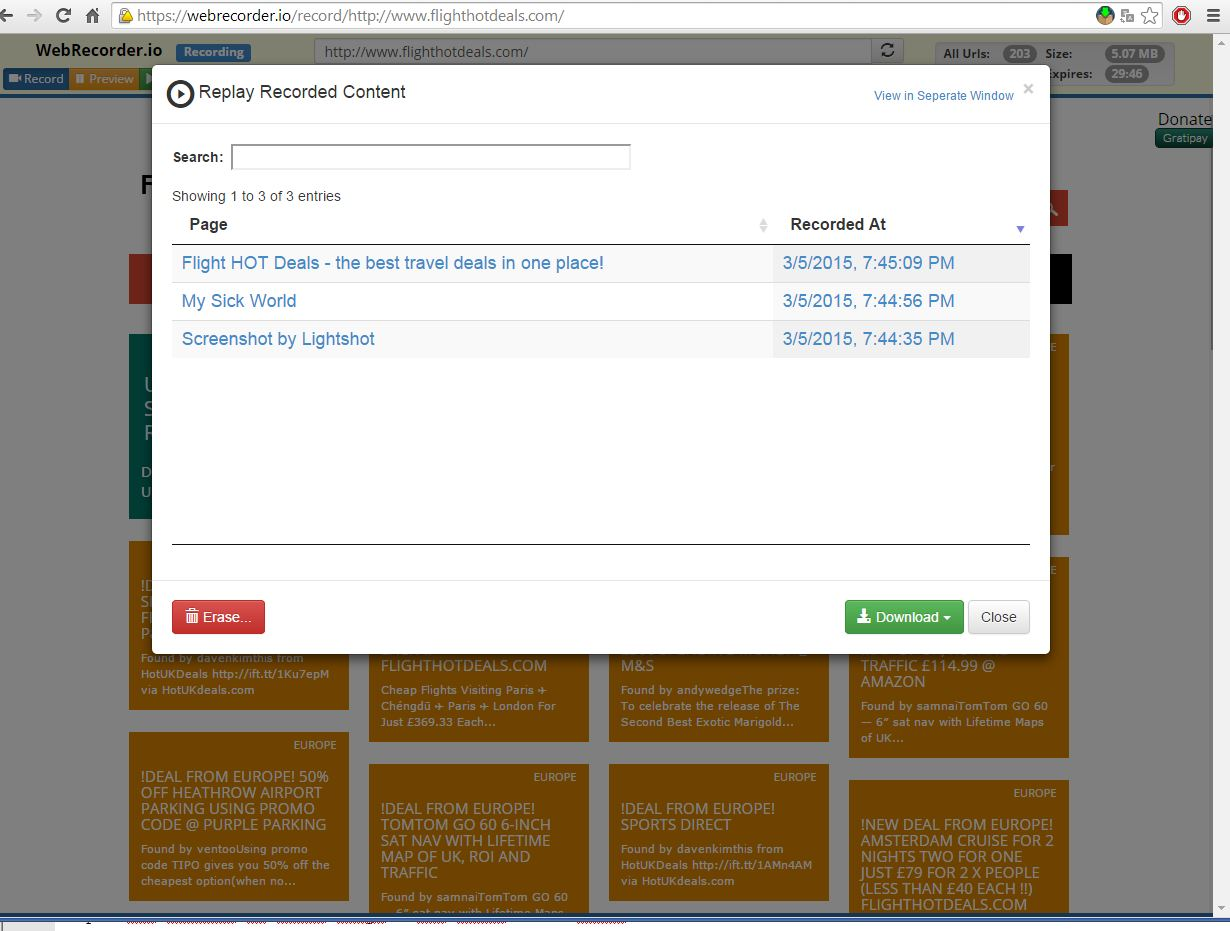
\includegraphics[scale=0.40]{webrecorderWarc.jpg}
		  	 		\caption{Generating warc files for multiple URIs using webrecorder}
			  \end{center}
		  \end{figure}	
	\item Quantitative comparison of WARC files generated by WAIL,webrecorder,WARCreater and wget is done on the basis of sizes.
	\item The comparison sizes are WAIL= 40 MB , webrecorder = 20.48 MB, WARCreate = 15.36 MB, wget = 4 MB.
	\item The WAIL size is more compared to others because WAIL software crawls data of the links in the website.
	\item This comparison is shown in the graph below.
	
	\begin{figure}
		  	 \begin{center}
		  	 		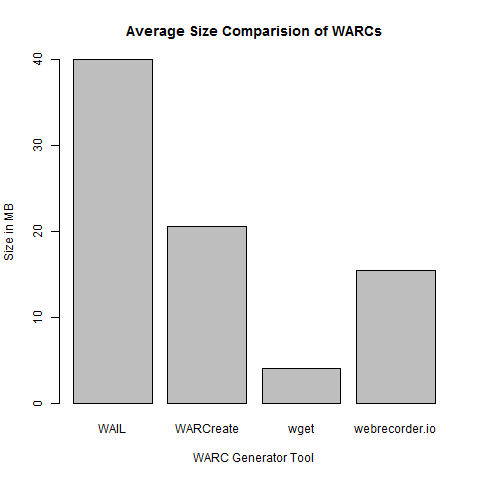
\includegraphics[scale=0.40]{Sizehistogram.png}
		  	 		\caption{Average Size Comparision of WARC}
			  \end{center}
	\end{figure}	
	\item Installed pywb to playback warc files. 
	\item pywb requires cdx for each warc to playback,so generated cdx file for each warc file.	
	\item I have put all my warc files into a new folder and changed the archivepaths of config.xml to point my warc files.
	\item Play back for two warc files using pywb is shown in the below figure.
	\item The WARC file which was in the play back does not have some images and some urls. 		
		\begin{figure}
		  	 \begin{center}
		  	 		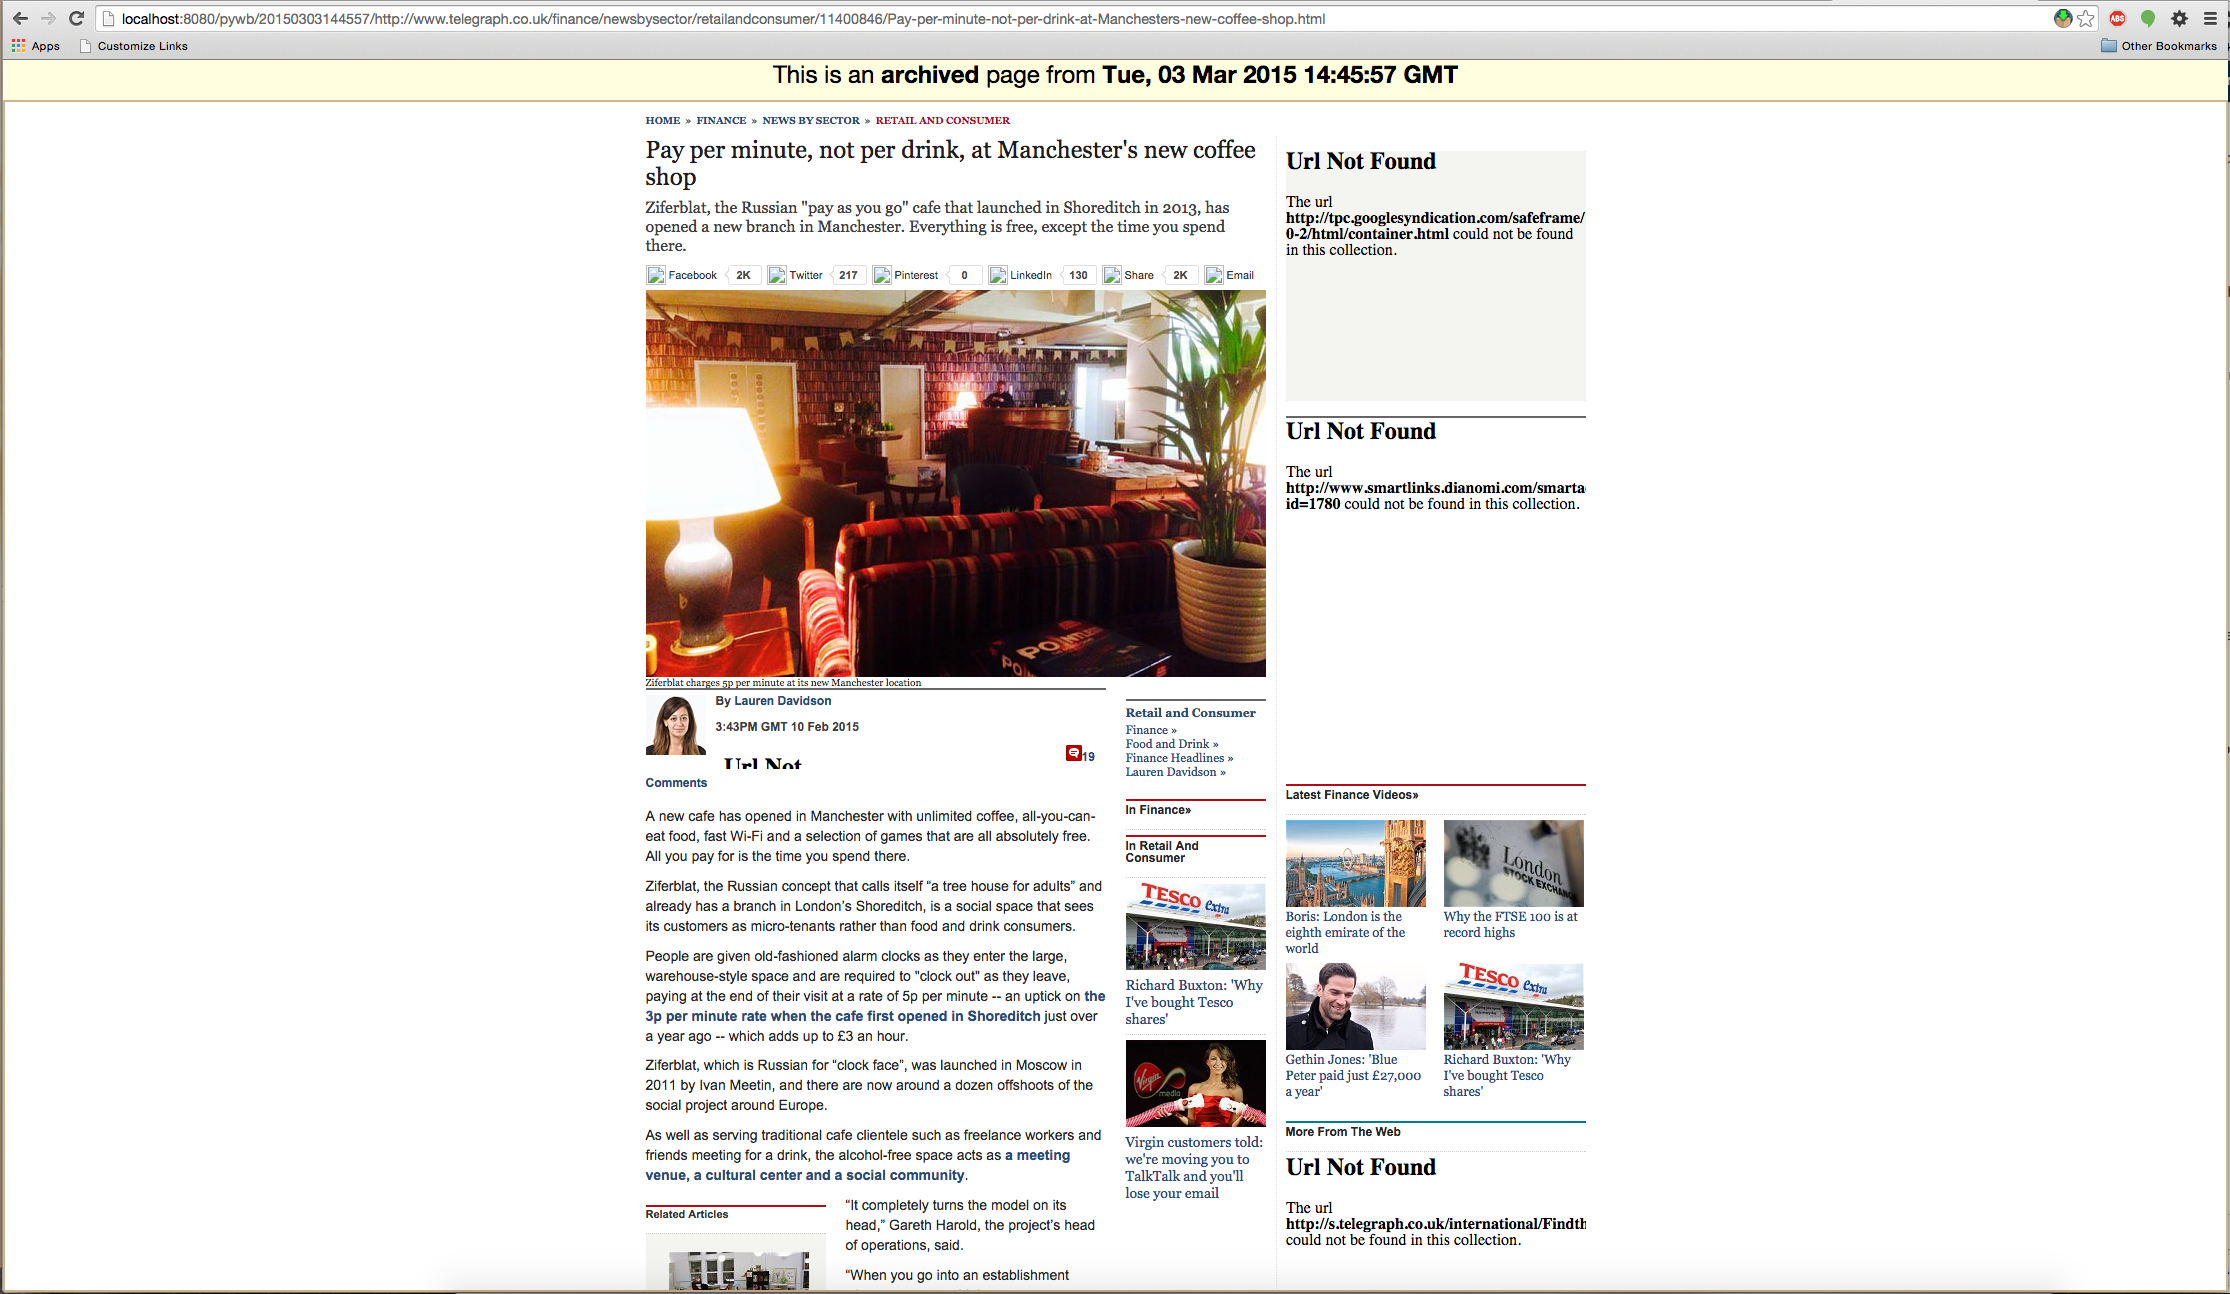
\includegraphics[scale=0.40]{pywbplayback.png}
		  	 		\caption{Play back warc file using pywb}
			  \end{center}
		  \end{figure}	
	\item The WARC file which is in the play back does not contain certain CSS archives and some links
		  \begin{figure}
		  	 \begin{center}
		  	 		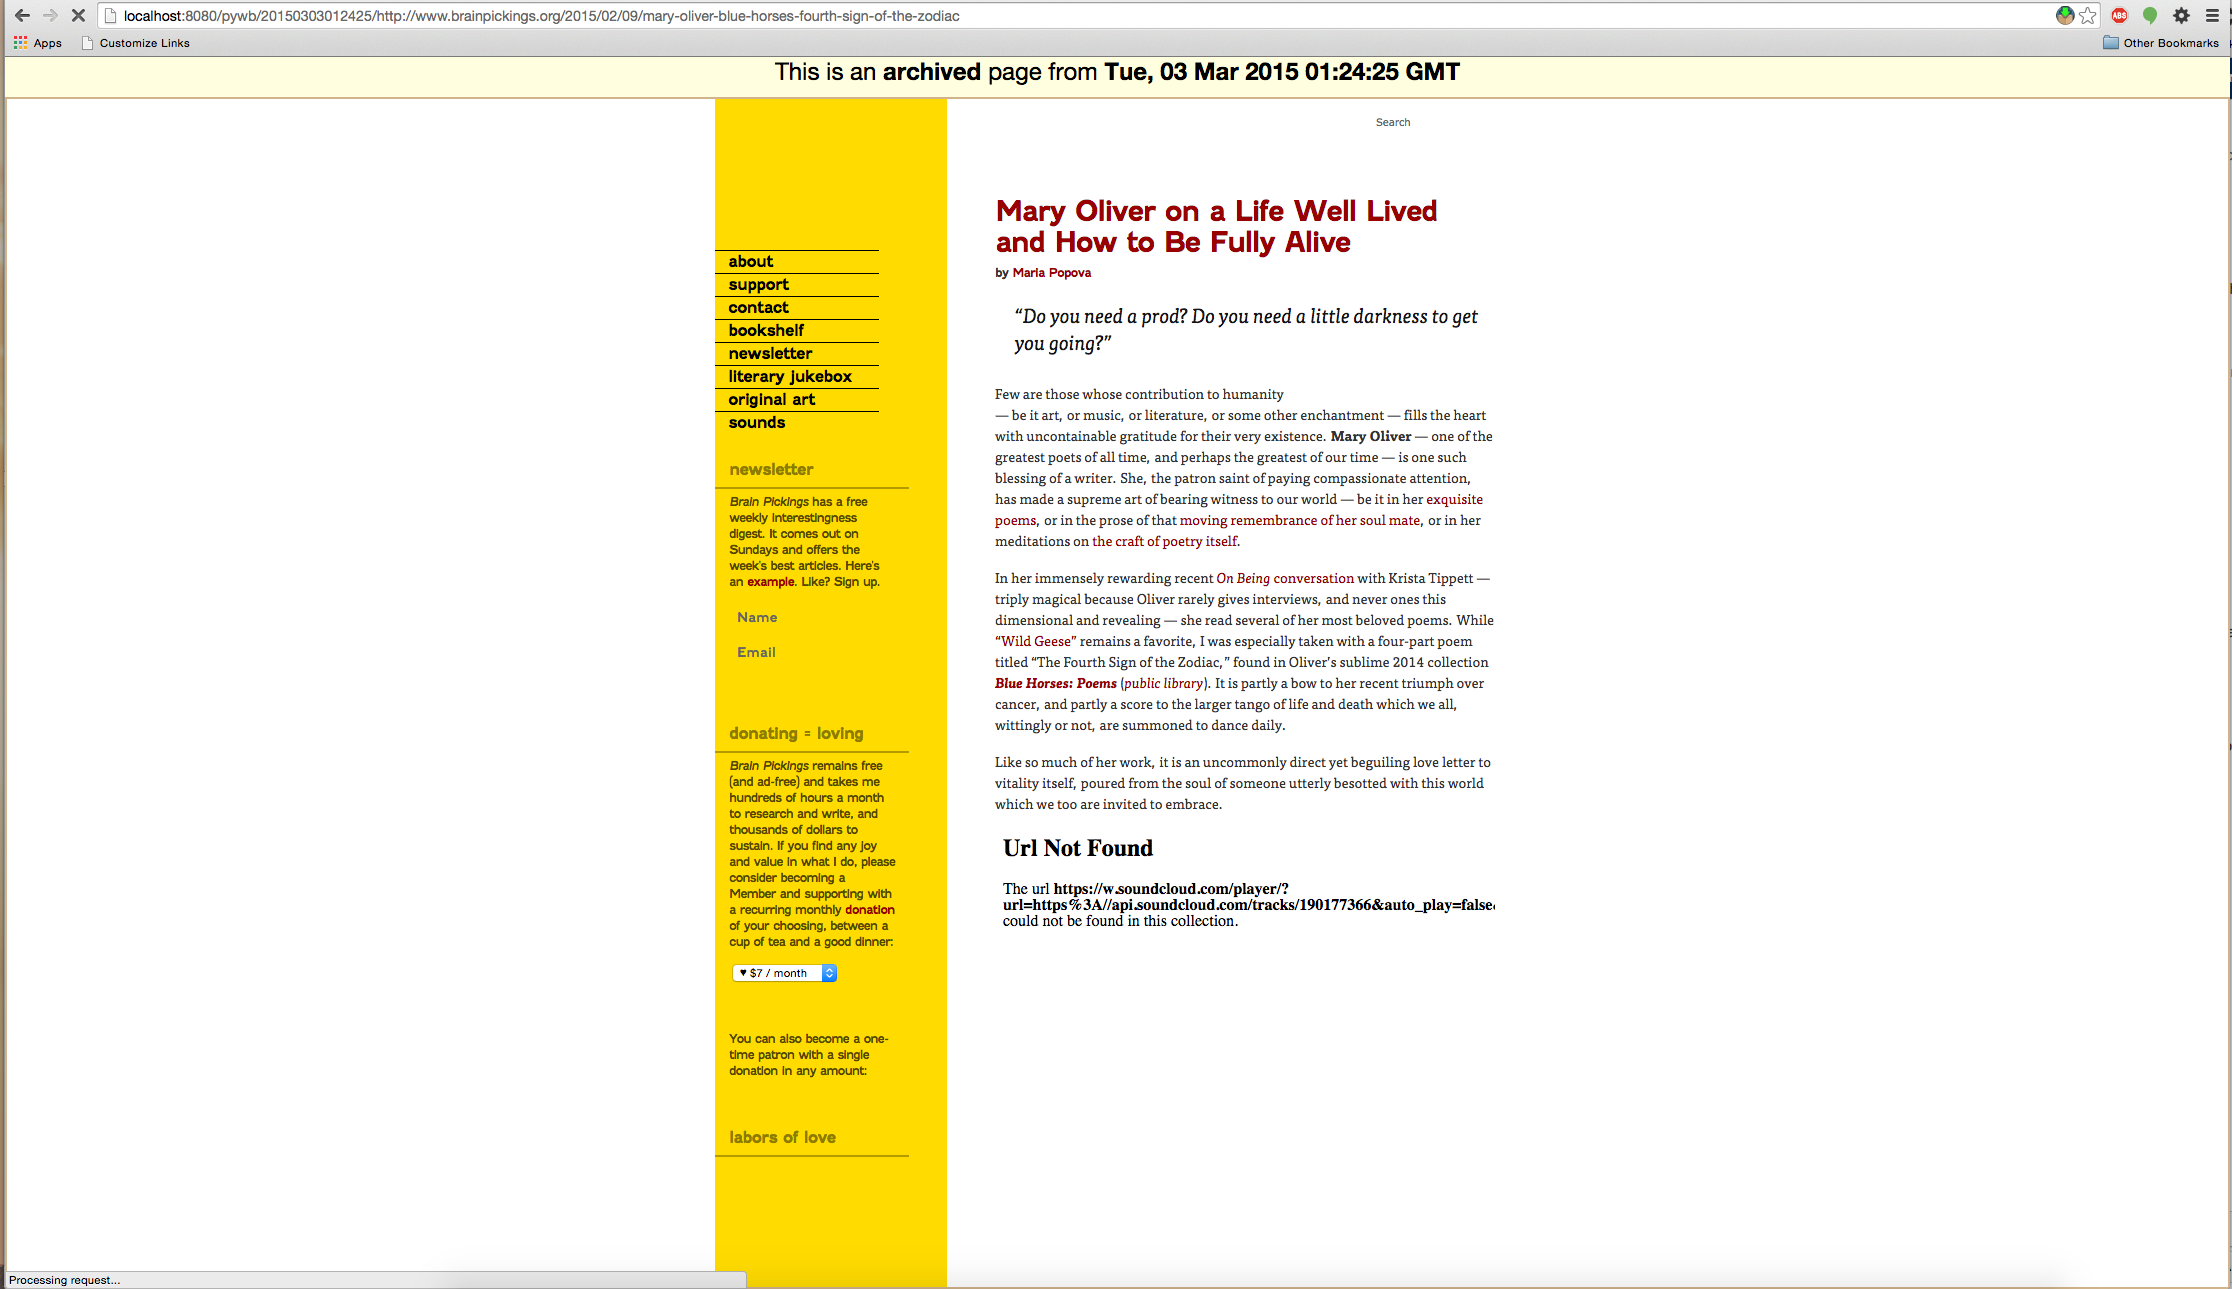
\includegraphics[scale=0.40]{pywbplayback2.png}
		  	 		\caption{Play back warc file using pywb}
			  \end{center}
		  \end{figure}
	\item WebRecorder.io takes warc file to replay the archived file. Play back for two warc files using WebRecorder.io is shown in the below figure
	\item The WARC file in this play back worked perfectly without any faults.		
		\begin{figure}
		  	 \begin{center}
		  	 		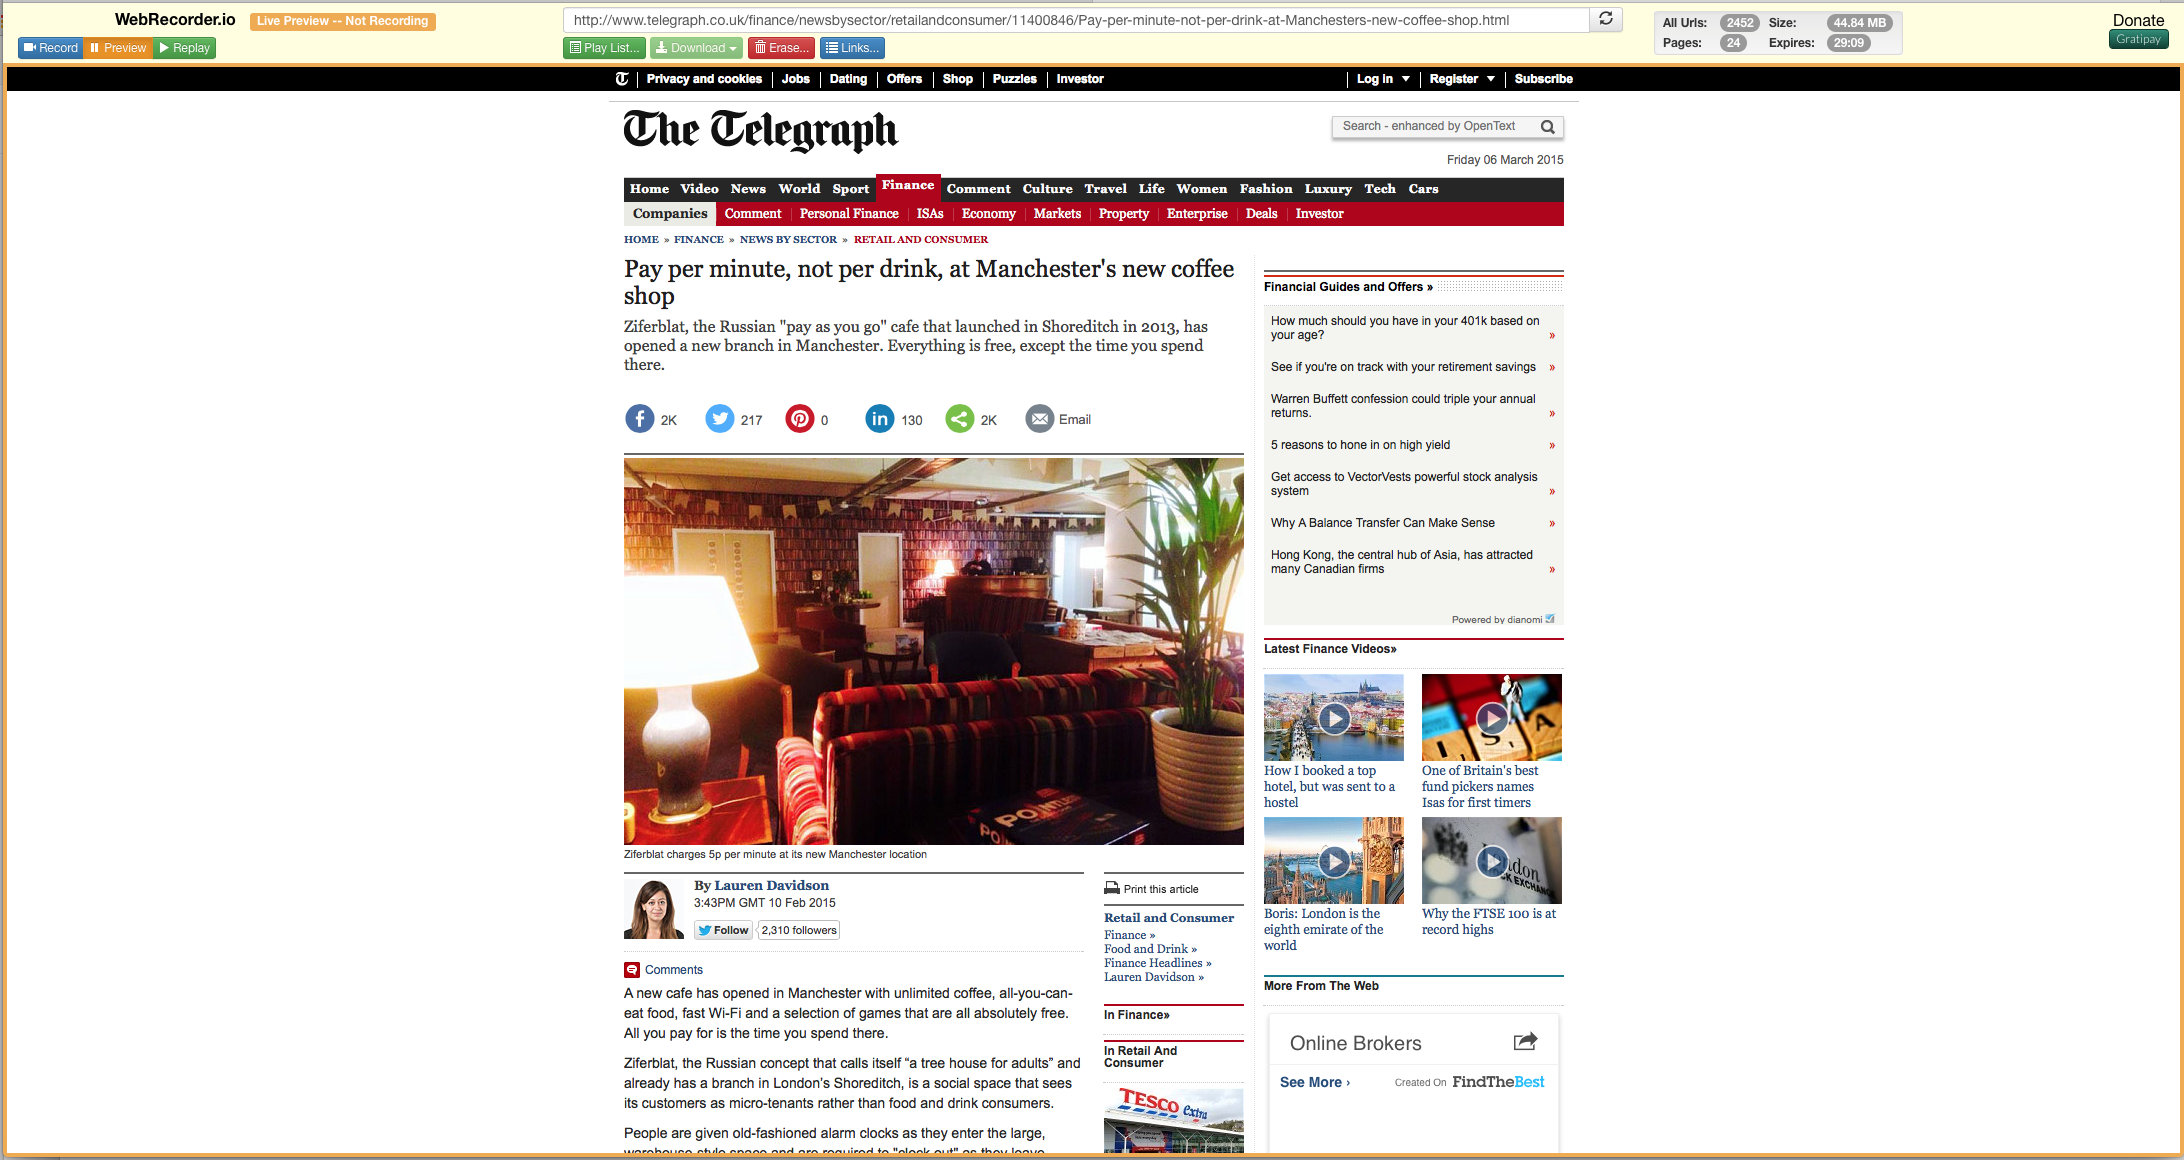
\includegraphics[scale=0.40]{webrecorderplayback.png}
		  	 		\caption{Play back warc file using webrecorder}
			  \end{center}
		  \end{figure}	
	 \item The WARC file in this play back did not have certain images.
		  \begin{figure}
		  	 \begin{center}
		  	 		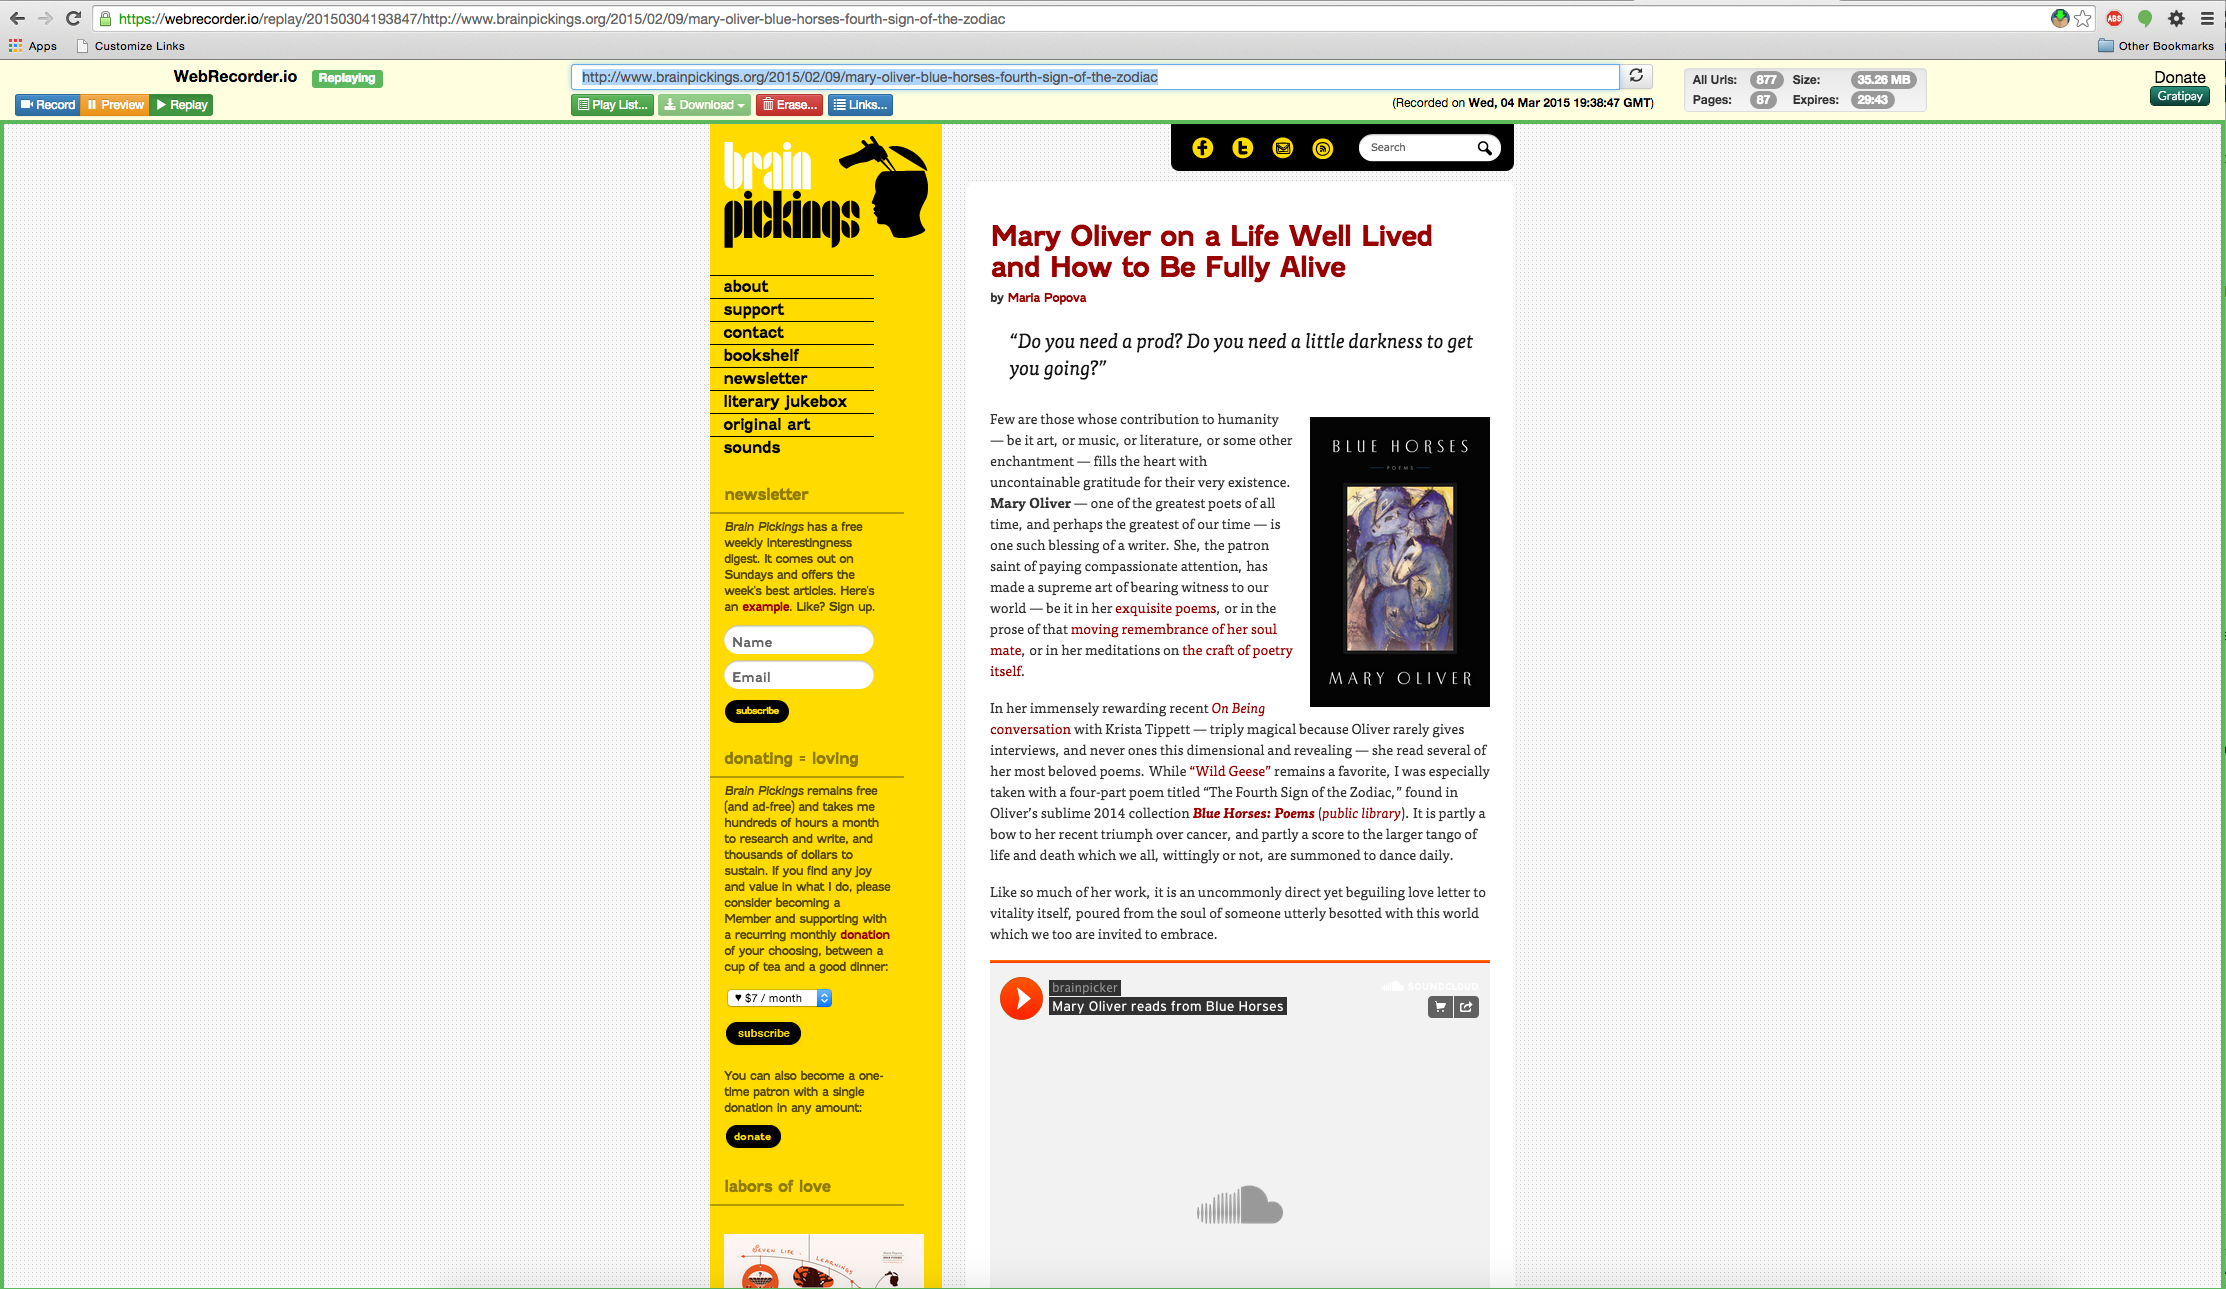
\includegraphics[scale=0.40]{webrecorderplayback2.png}
		  	 		\caption{Play back warc file using webrecorder}
			  \end{center}
		  \end{figure}	
	
\end{itemize}
\newpage
